\chapter{El Proyecto}


\section{Motivaci\'on}

En la actualidad existen pocos sistemas Aplicados en el \'ambito de la gesti\'on en
el area de Medicina y los existentes suelen ser solo para areas especificas


\section{Descripci\'on del Proyecto}

Lo que se pretendi\'o con este proyecto era poder desarrollar un sistema que unifique
la areas de gesti\'on y asignaci\'on de turnos y el manejo de historia cl\'{\i}nica en 
un \'unico sistema.

Cabe aclarar que el mismo se desarrollo con el prop\'osito de poder ser utilizado 
principalmente en policonsultorios m\'edicos ya que no plantea cuestiones tales como
internaciones, traslado de pacientes, etc. como para poder ser de correcta utilidad
en cl\'{\i}nicas y hospitales. 


\section{Arquitectura de la Aplicaci\'on}

Implementado en Python utilizando en Framework Django, utilizando el motor de bases
de datos PosgreSQL, funciona con una interfaz web por lo que se se accede al
mismo mediante un Navegador Web, Internamente maneja 2 Modulos principales
que son el  ``Modulo de Gesti\'on de Turnos" y el ``Modulo de manejo de
Historia Cl\'{\i}nica" , al ser un sistema web implementa un tercer modulo de manera
impl\'{\i}cita que control de acceso mediante la definici\'on de Grupos Usuarios y
sus correspondientes permisos.


\section{Modulo Usuarios}

La gesti\'on de usuarios es un proceso bastante com\'un en casi todos los sistemas,
muchos desarrolladores terminan programando funcionalidades de autenticaci\'on 
una y otra ves a lo largo de los a\'nos y casi siempre funcionando de la misma 
manera. Django se pens\'o para simplificar la vida no para complicarla, por eso
al ser una tarea bastante com\'un en casi todas las aplicaciones, viene incluido
un completo sistema de autenticaci\'on que gestiona:

\begin{itemize}
    \item Usuarios
    \item Grupos
    \item Permisos
    \item Sessiones de Usuarios y Cookies
\end{itemize}

Aunque en cuanto a lo que se refiere manejo de sesiones es un completo sistema
solo maneja un peque\~no conjunto de datos por lo que hubo que extender mediante 
la adici\'on de un Modelo adicional para complementar la informaci\'on de los 
usuarios.


\subsection{Modelos}

Aqui un diagrama con todos los modelos que componen el modulo Usuarios.

\begin{figure}[H]
    \centering
    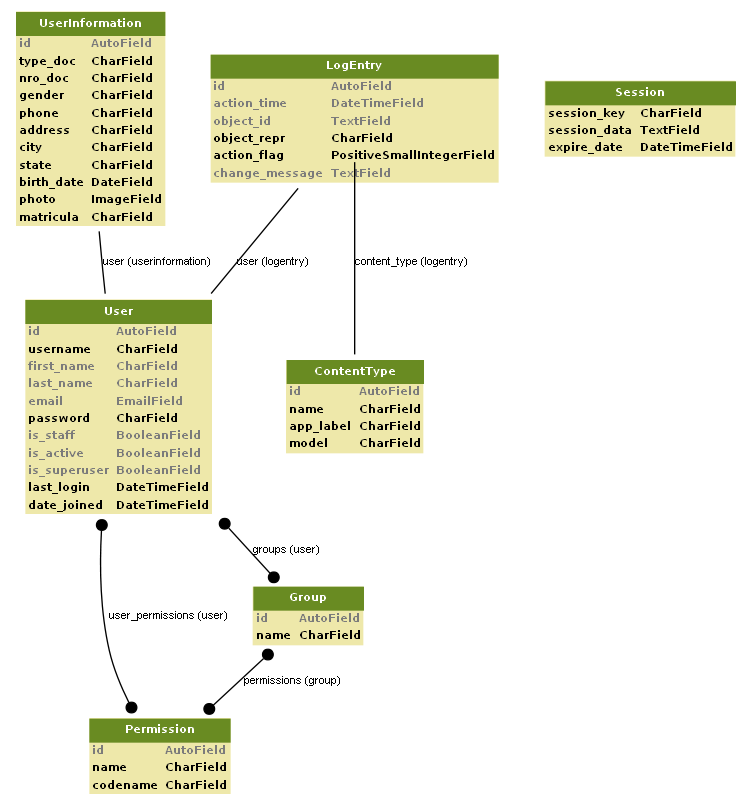
\includegraphics[scale=0.6]{resourse/auth.png}
    \caption{Diagrama con modelos que componen el modulo Usuarios}
    \label{fig:07}
\end{figure}

Si lo expres\'aramos mediante la notaci\'on UML para Diagramas de Clases 
tendr\'{\i}amos lo siguiente.

\begin{figure}[H]
    \centering
    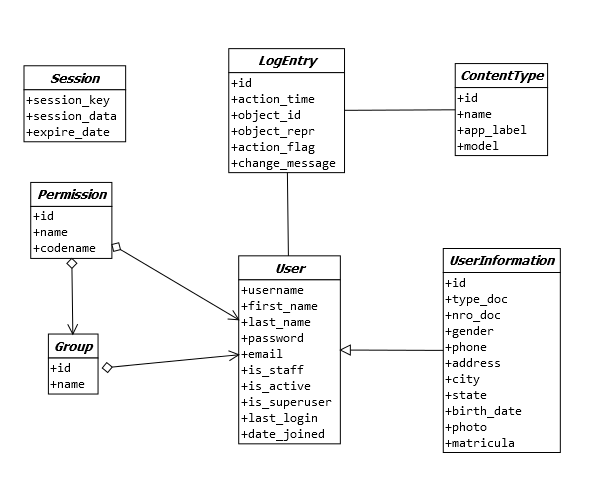
\includegraphics[scale=0.7]{resourse/uml-users.png}
    \caption{Diagrama con modelos que componen el modulo Usuarios}
    \label{fig:07}
\end{figure}

El \'unico modelo que fue necesario agregar es UserInformation el resto vienen
con Django. En Resumen aunque se podr\'{\i}a haber desarrollado Un Modulo desde
cero que gestione las sesiones de usuarios hubiese generado trabajo extra sin
sentido.

\subsection{Usuarios y Permisos}

El sistema contempla 4 tipos de usuarios los cuales son: 

\begin{itemize}
    \item Usuarios no registrados 
    \item Pacientes
    \item M\'edicos
    \item Administrativos
\end{itemize}

\subsubsection{Usuarios no Registrados}

Los \textbf{Usuarios no registrados} que vendr\'{\i}a a ser cuando el usuario ingresa
a la aplicaci\'on y no hay ninguna sesi\'on iniciada, pueden acceder al sistema para 
consultar informaci\'on b\'asica y horarios de atenci\'on de los especialistas que 
forman parte de la instituci\'on, adem\'as de tener la opci\'on de registrarse 
como paciente.\\[0.1cm]    

\subsubsection{Paciente}

El rol \textbf{Paciente} corresponde a los usuarios comunes, un usuario paciente puede 
ser creado por cualquiera de los otros roles, en caso que sea un usuario no registrado
quien da el alta como paciente, el mismo deber\'a confirmar el registro mediante un
codigo de verificaci\'on que el sistema le enviara al correo antes de poder comenzar
a usar su cuenta, en los otros casos (el usuario Paciente es registrado por un 
medico o un Administrativo) no se requerida dicha confirmaci\'on.\\[0.1cm]

En cuanto a los privilegios del usuario Paciente, este adem\'as de poder consultar la 
la informaci\'on de los especialistas puede solicitar un turno para ser atendido 
a un especialista en particular, tambi\'en realizarle una interconsulta (mediante
el sistema interno de mensajer\'{\i}a) y modificar sus datos b\'asicos, en resumen sus 
posibles funciones son:


\subsubsection{Medico}

Los Usuarios \textbf{M\'edicos} los cuales son asignados por los Administrativos a 
los Especialistas, en cuanto a privilegios y funcionalidades dentro del sistema, 
los mismos pueden:

\begin{itemize}
    \item Registrar Pacientes
    \item Modificar datos de Pacientes
    \item Enviar Mensajes a cualquier Usuario
    \item Registrar Turnos 
    \item Cancelar Turnos
    \item Administrar sus Horario de Atenci\'on
    \item Cancelar d\'{\i}as de atenci\'on
\end{itemize}

Son los \'unicos usuarios que tienen acceso al Modulo \textit{Historia Clinina}, en cuanto
a privilegio sobre este modulo diremos que tiene la posibilidad de Crear,Modificar,
Borrar (salvo casos espec\'{\i}ficos, que por su naturaleza no se permite dicha 
modificaci\'on.) un conjunto de Estudios, para mas detalle se recomienda consultar
el apartado sobre tal modulo.


\subsubsection{Administrativo}

En cuanto a los usuarios \textbf{Administrativo} poseen los mismos permisos que 
un usuario \textbf{Medico} exceptuando que no poseen acceso a las funcionalidades 
del Modulo Historia Cl\'{\i}nica, como privilegio especial pueden administrar las 
cuentas de usuario de todos los roles incluidos en el sistema, incluido los 
Medico y otros Administrativos.

\subsubsection{Admin}

Existe un rol adicional que Django crea y gestiona por aparte, el mismo queda 
delegado para los administradores del sistemas ya que mediante el se puede acceder
y modificar cualquier parte de la base de datos, por lo que podr\'{\i}amos decir que 
es un \textbf{Super Usuario}, o usuario \textbf{Root} como para hacer analog\'{\i}a
con los usuarios en entornos Unix, el mismo no forma parte del sistema desarrollado
sino como funcionalidad adicional Django provee un panel de administraci\'on, 
para dicho tipo de usuario, al cual se puede acceder desde \url{/admin/} por ejemplo
si estuvi\'esemos ejecutando en un servidor local la ruta completa seria 
\url{http://127.0.0.1/admin/}\footnote{Se puede consultar mas acerca de Django
Admin en \url{https://docs.djangoproject.com/en/dev/ref/contrib/admin/}}.\\[0.1cm]


\begin{figure}[h]
    \centering
    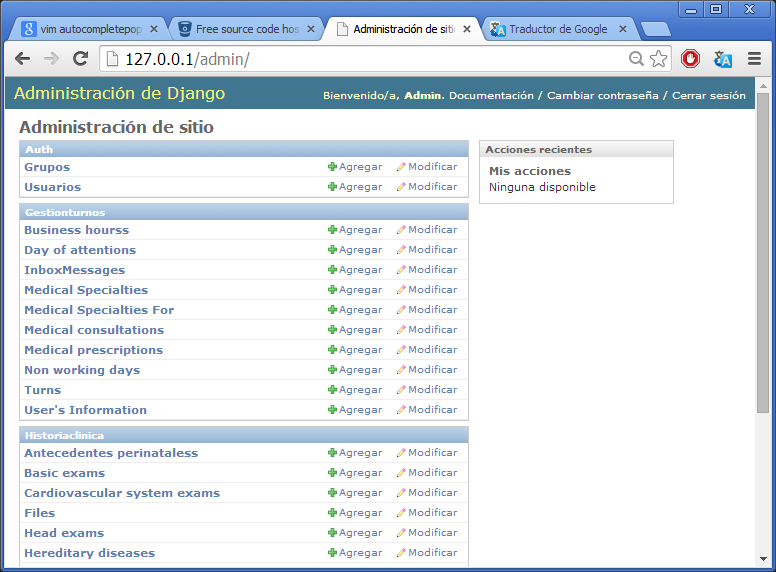
\includegraphics[scale=0.5]{resourse/django-admin.png}
    \caption{Vista del Panel Administracion provisto por Django}
    \label{fig:123}
\end{figure}  


Cabe aclarar que el Super Usuario del sistema de Autenticaci\'on de Django dentro 
del sistema en si mismo no posee ning\'un privilegio adicional, es mas para 
compatibilizar el usuario con la funcionalidad del sistema, cuando se inicializan
por primera ves, se crea un usuario de este tipo llamado \textbf{admin} al cual
se le asignan privilegio de \textit{Administrativo}.


%%%%%%%%%%%%%%%%%%%%%%%%%%%%%%%%%%%%%%%%%%%%%%%%%%%%%%%%%%%%%%%%%%%%%%%%%%%%%%%

\section{Modulo Gesti\'on de Turnos}

Dejando de lado el modulo Usuarios que nos provee Django el sistema desarrollado 
se divide esencialmente en 2 partes o m\'odulos, aqu\'{\i} explicare como se dise\~no e
implemento el Modulo Gesti\'on de Turnos, que a mi consideraci\'on fue el que mayor
reto aporto a la hora de pensar un soluci\'on para poder implementarlo.

El modulo se encarga de implementar las siguientes funciones

\begin{itemize}
    \item Gestionar Datos de Usuarios
    \item Mensajer\'{\i}a Interna
    \item Asignacion de Especialidades Medicas
    \item Asignaci\'on de Turnos
\end{itemize}



\subsection{Definicion del Modelo}

Aqui se muestra el diagrama de modelos que componen el modulo \textbf{Gestion 
de Turnos} \footnote{Vuelven a aparecen los modelos User y UserInformation por 
que casi todos los otros modelos dependen de alguna forma de ellos}, por la 
cantidad de modelos se mostrara en 2 diagramas, igualmente tengase en cuenta
que corresponden a un unico modelo, lo que haremos sera separar en los modelos
especificos utilizados para gestion de turnos y el resto de los modelos 
definidos que complementan la funcionalidad del modulo.


\begin{figure}[h]
    \centering
    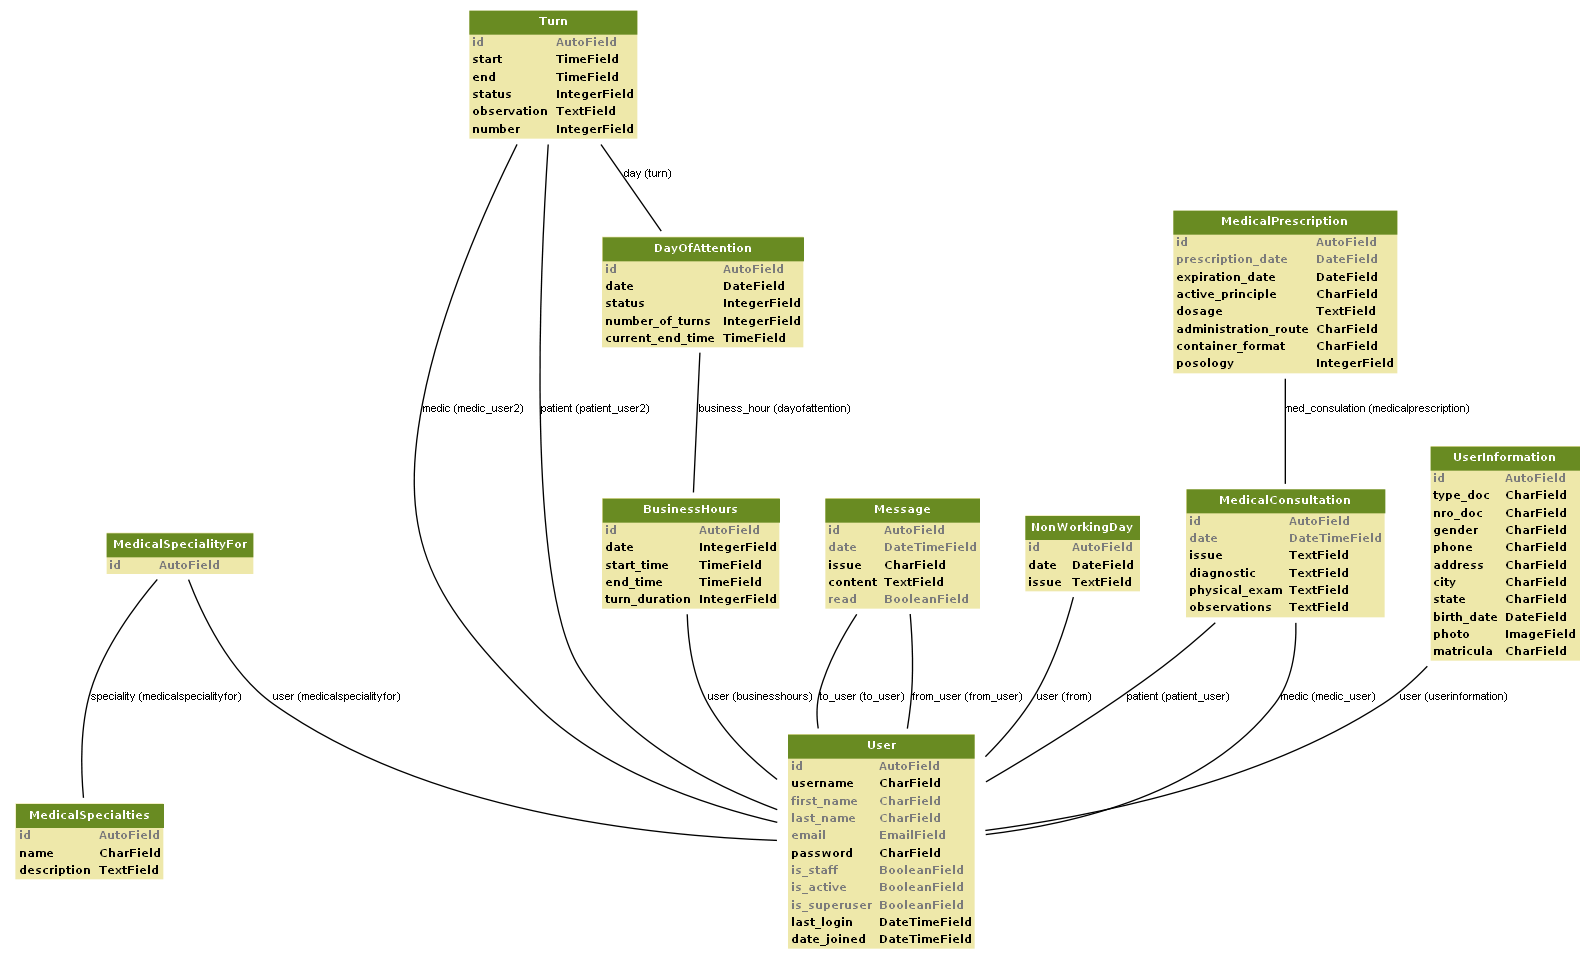
\includegraphics[scale=0.5]{resourse/gestionturnos-class-diagram.png}
    \caption{Vista del Panel Administracion provisto por Django}
    \label{fig:123}
\end{figure}  


\subsection{Gestionar Datos de Usuarios}

Esta funcionalidad describe, todo lo referido a la alta, baja y modificaci\'on de 
los datos de todos los usuarios. Implementa las vista tanto para modificacion de 
datos personales, vistas de administrador para gestionar datos de otros usuarios. 


\subsection{Mensajer\'{\i}a Interna}

Permite la comunicacion interna entre los usuarios, su principal utilidad es 
permitir que los Pacientes puedan realizar peque\~nas interconsultas a los 
medicos atraves de la plataforma, sin requerir una consulta medica.

\subsection{Asignacion Expecialidades Medicas}

Dentro el modulo permite asignarles especialiades medicas correspondientes a 
a los profesionales, aunque no realiza una distincion especifica a la hora de 
asignar turnos, simplemente considera que el medico en dicho horario puede 
atender cualquier consulta relacionada a sus especializaciones. \footnote{
Tengase en cuenta que es raro ver un medico con varias especializaciones Medicas
y que el sistema fue pensado para ser utilizado en un consultorio medico, donde
no se suele contar con equipamiento de alta complejidad.}

\subsection{Asignaci\'on de Turnos}  

Es la principal funcionalidad del modulo, que permite:

\begin{itemize}
    \item Definir dias de atencion
    \item Asignar dias en los cuales no se atendera     
    \item Asignar turnos
    FALTA ESPECIFiCAR BIEN ..!
\end{itemize}


\\[0.5cm]

\subsection{Dise\~no de Modelos Para la Gestion de Turnos}

Aqui se muestran los algunas consideraciones que se tubieron en cuenta a la hora de 
dise\~nar los modelos para implementar la funcionalidad de asignacion de turnos
propiamente dicha la cual define el nombre del modulo. 

\subsubsection{BussinesHour(Horario De Atencion)}

Este modelo se utiliza para definir el horario de atencion de cada medico, en 
el se especifican parametros como:

\begin{itemize}
    \item \textbf{user}: referencia al medico al cual pertence 
    \item \textbf{date}: define el dia de atencion \footnote{Esto hace 
        referencia a los dias de la semana osea Lunes, Martes,..., etc. por el 
        momento solo se puede definir un unico dia de atencion por dia por 
    medico.}
    \item \textbf{start\_time, end\_time}: marca el horario de inicio y fin del 
        dia de atencion del medico.
    \item \textbf{turn\_duration} duracion estimada del turno
\end{itemize}

En base a esto se puede calcular un dato adicional que es la cantidad de turnos
que se pueden asignar en tal dia, y se hace de la siguiente manera:

\begin{lstlisting}
numero\_turnos = (hora\_fin - hora\_inicio) // turn\_duration
\end{lstlisting}

Esto devolvera un valor entero, que sera el numero maximo de turnos que se 
puedan asignar.


\subsubsection{DayOffAttention (Dias de Atencion)}

Este modelo maneja la disposicion horaria de una fecha en particular, se basa 
en los datos que se definieron en el modelo anterior BussinesHour, por lo que 
solo se pueden generar en las fechas que correspondan con los dias de la semana
asignados, cuenta con los siguientes parametros:

\begin{itemize}
    \item \textbf{bussines\_hour}: referencia al horario de atencion definido 
        por el medico.
    \item \textbf{date}: que fecha cae ese dia, esto se refiere al dia del a\~no 
        especifico.
    \item \textbf{status}: informacion del estado del dia, es de tipo booleano
        y especifica el estado del dia de atencion siendo el valor true 
        para explicar que se pueden asignar mas turnos y FALSE que no se 
        pueden asignar mas. \footnote{ Que un dia de atencion este marcado como 
        no disponible (status=FALSE) puede significar que el cupo este lleno o 
        que ese dia el medico no pueda asistir o sea feriado por ejemplo, para 
        determinar de que se trata si dice no disponible y no hay ningun turno 
        asignado (number\_of\_turns=0) significara que ese dia el medico no 
        atiende }
     \item \textbf{number\_of\_turns}: numero de turnos que van siendo asignados
     \item \textbf{current\_end\_time}: horario actual de finalizacion 
\end{itemize}


\subsubsection{Turn (Turno)}

Este modelo se define para registrar la informacion correspondiente a los 
turnos asignados es dependiente del modelo anterior (DayOffAttention) donde se 
especifican el resto de los datos como la fecha.

En cuanto a sus atributos, mucho no hay que explicar y son:

\begin{itemize}
    \item \textbf{day}: hace referencia a un dia de atencion (DayOffAttention)
    \item \textbf{medic}: referencia a los datos del medicos
    \item \textbf{patient}: referencia al paciente. 
    \item \textbf{start, end}: hacen referencia a las horas de inicio y fin 
        correspondientemente.
    \item \textbf{status}: estado del turno es de tipo enumerado define varios 
        posibles estados entre los que estan (pendiente, concretado, cancelado 
        medico, cancelado paciente).
    \item \textbf{observation}: campo de texto, para registrar cualquier 
        observacion pertinente.
    \item \textbf{number}: se refiere al numero de orden para atencion.
\end{itemize}

\subsubsection{Consideraciones}

En cuanto a funcionamiento de la asignacion de turnos se tienen en cuenta las
siguientes consideraciones: \\[0.1cm]

Un turno no puede ser cancelado despues de su hora de inicio por el paciente, 
siendo asi posible de ser cancelado por el medico. \\[0.1cm]

Al ser cancelado por un paciente se debe cambiar correspondiente estado dentro 
de dia de atencion. \\[0.1cm]

 Si un medico cancela un turno el mismo no se modificara el estado en la tabla 
 dia de atencion, como el caso de los paciente que cancelen un turno, 
 para el sistema hara de cuenta que los mismo ocurrieron, aunque si un turno es 
 cancelado por el medico el mismo no sera reprogramado.

 En todos los casos los usuarios deverian poder recivir el correspondiente 
 notificacion de que se cancelo dicho turno invitandolos a reprogramar el mismo.

Los pacientes no pueden solicitar turnos durante el horario de atenci\'on del 
mismo, si el servidor comprueba que existen turnos sin actualizar estado como 
pendientes, si el medico o administrador no actualizo los msmos y ya paso la 
hora del mismo tiene que enviar notificaciones correspondientes. 



\section{Modulo Historia Cl\'{\i}nica}

Este modulo del sistema tiene como tarea manejar y recolectar toda informaci\'on 
referente a las historia cl\'{\i}nica de los pacientes.


\subsection{?`Que es una Historia Cl\'{\i}nica?}

Antes de entrar en todo lo referente sobre el desarrollo del correspondiente modulo
tomo un momento para explicar concretamente a que no referimos cuando hablamos de 
la misma por lo que aqu\'{\i} tenemos la siguiente definici\'on:

La historia cl\'{\i}nica es un documento m\'edico-legal que surge del contacto entre el 
profesional de la salud (m\'edico, pod\'ologo, psic\'ologo, asistente social, enfermero, 
kinesi\'ologo, odont\'ologo, etc.) y el paciente donde se recoge la informaci\'on necesaria 
para la correcta atenci\'on de los pacientes. La historia cl\'{\i}nica es un documento 
v\'alido desde el punto de vista cl\'{\i}nico y legal, que recoge informaci\'on de tipo 
asistencial, preventivo y social.

La Historia Cl\'{\i}nica se origina con el primer episodio de enfermedad o control de salud en 
el que se atiende al paciente, ya sea en el hospital o en el centro de atenci\'on primaria, 
o en un consultorio m\'edico. La historia cl\'{\i}nica est\'a incluida dentro del campo de la 
semiolog\'{\i}a cl\'{\i}nica \footnote{La Semiolog\'{\i}a Cl\'{\i}nica es el cuerpo del conocimiento
que se ocupa de la identificaci\'on de las diversas manifestaciones patol\'ogicas 
\cite{SemiClin}}.

\subsection{La Historia Cl\'{\i}nica en la Ley Argentina}

La documentaci\'on m\'edica comprendida en lo que com\'unmente se denomina ``historia 
cl\'{\i}nica" la cual no se encontraba regida por leyes especificas en la Argentina hasta
el 19 de noviembre del 2009 donde se promulga la Ley 26.529 \cite{LeyHC}.

En el cap\'{\i}tulo primero de la ley sen enumeran los derechos de los pacientes, 
en el art\'{\i}culo 2, inciso ``a". Renueva el derecho a la intimidad y la confidencialidad, 
donde se hace hincapi\'e sobre la responsabilidad de preservar la intimidad y 
confidencialidad de toda la documentaci\'on m\'edica concerniente a los pacientes, 
particularmente el inciso ``d" del mismo art\'{\i}culo:

``El paciente tiene derecho a que toda persona que participe en la elaboraci\'on 
o manipulaci\'on de la documentaci\'on cl\'{\i}nica, o bien tenga acceso al contenido de 
la misma, guarde la debida reserva, salvo expresa disposici\'on en contrario 
emanada de autoridad judicial competente o autorizaci\'on del propio paciente"

Garantiza adem\'as el respeto por la autonom\'{\i}a del paciente y el derecho a recibir 
la informaci\'on necesaria para su salud, incluyendo el derecho a negarse a ser 
informado.

El cap\'{\i}tulo III reza sobre el Consentimiento Informado, el cual est\'a basado en 
el principio de autonom\'{\i}a, es decir, el derecho del paciente a ser reconocido 
como persona libre y due\~na de tomar sus decisiones. Para ello el paciente debe estar en 
condiciones de comunicar su decisi\'on y  \'este ha sido informado adecuadamente de 
sus opciones, es decir, no pueden ser decisiones hechas como resultado de delirio 
o alucinaciones. La decisi\'on del paciente es consistente con sus valores y metas 
y se mantiene estable en el tiempo si no han habido modificaciones hechas por
el mismo sujeto. Los familiares de un paciente no est\'an en el derecho de 
requerir al m\'edico del paciente que no se le comunique ciertos detalles o
informaci\'on al mismo. 

Ahora bien vallamos a lo que nos interesa:

La ley define a la Historia Cl\'{\i}nica como el documento ``obligatorio, cronol\'ogico,
foliado y completo en el que consta toda actuaci\'on realizada al paciente por
profesionales y auxiliares de la salud." Define que la historia cl\'{\i}nica es 
propiedad del paciente, siendo este el titular de la misma. Siempre que un paciente 
solicite la historia cl\'{\i}nica, la instituci\'on competente debe entregarle una copia
autenticada en 48 horas. Si no es entregada en ese plazo, el
paciente est\'a autorizado a interponer un recurso de Habeas Data, juzgado de por 
medio. 

Entre los datos que han de consignarse en forma obligatoria esta la fecha de 
inicio y confecci\'on de la historia cl\'{\i}nica, datos identificatorios del paciente
y su n\'ucleo familiar, datos del profesional interviniente y su especialidad, 
registros claros y precisos de los actos realizados por profesionales y auxiliares
intervinientes, antecedentes gen\'eticos, fisiol\'ogicos y patol\'ogicos si los hubiere,
y todo acto m\'edico realizado o indicado.

Incluye en la historia cl\'{\i}nica a todos los documentos que hagan referencia a 
informaci\'on de salud del paciente, a\~nadiendo los consentimientos informados, 
hojas de indicaciones, hojas de enfermer\'{\i}a, estudios complementarios, 
incluyendo las``pr\'acticas realizadas, rechazadas o abandonadas." 
Esto  \'ultimo es interesante: si el paciente abandona o rechaza un tratamiento 
propuesto, es responsabilidad del m\'edico consignarlo, que a fin de cuentas es el
beneficiario de que aquello quede asentado desde el punto de vista m\'edico-legal.

Autoriza a reclamar una copia de la historia cl\'{\i}nica al paciente y su representante 
legal, al c\'onyuge o conviviente de hecho (sin importar el sexo), y a los herederos 
forzosos. Lo que no queda claro del art. 19 inciso b es si los c\'onyuges y 
convivientes requieren o no la autorizaci\'on del paciente.

Se a\~nade esta ley al cap\'{\i}tulo 11 del C\'odigo de \'etica de la Asociaci\'on M\'edica 
Argentina, del a\~no 2001. En ella se explaya en forma m\'as extensa y detallada sobre
la confecci\'on. Particular inter\'es debi\'eramos prestarle al art. 168:

``La historia cl\'{\i}nica ha de ser un instrumento objetivo y comprensible por terceros,
y no solo por quienes escriben en ella." A su vez, el art. 171 especifica que 
"debe ser legible, no debe tener tachaduras, no se debe escribir sobre lo ya 
escrito, no debe ser borrada, no se debe dejar espacios en blanco y ante una
equivocaci\'on debe escribirse ERROR y aclarar lo que sea necesario. No se debe a\~nadir
nada entre renglones."


\subsection{Funcionalidades}

Las funcionalidades que se implementan en correspondiente m\'odulos son solo
b\'asicas y comprenden la documentaci\'on practicas mas comunes dentro del area de la 
medicina, esto no implica que solo valla a servir para eso \'unicamente, por su 
extructura el modulo contempla la posibilidad de agregar nuevos componentes para 
estudios especificos que sean requeridos y que no hayan sido contemplados en el 
actual sistema.




\section{Elecci\'on de la metodolog\'ia de Programaci\'on}

